\documentclass[12pt]{article}

\usepackage[]{amsmath}
\usepackage[]{amsthm}
\usepackage[]{amsfonts}
\usepackage[]{amssymb}
\usepackage{blindtext}
\usepackage[a4paper, total={7.5in, 10in}]{geometry}
\usepackage{graphicx}
\usepackage{listings}
\usepackage{color}
\usepackage{array}
\usepackage{wrapfig}
\usepackage{hyperref}

\definecolor{dkgreen}{rgb}{0,0.6,0}
\definecolor{gray}{rgb}{0.5,0.5,0.5}
\definecolor{mauve}{rgb}{0.58,0,0.82}

\pagenumbering{arabic}
\let\cleardoublepage\clearpage


%% parameters for code snippets, etc (to put a keywords and smaller snippets inline, use \texttt{} tag
\lstset{frame=tb,
  language=Java,
  aboveskip=3mm,
  belowskip=3mm,
  showstringspaces=false,
  columns=flexible,
  basicstyle={\small\ttfamily},
  numbers=left,
  numberstyle=\small\color{black},
  keywordstyle=\color{blue},
  commentstyle=\color{dkgreen},
  stringstyle=\color{mauve},
  breaklines=true,
  breakatwhitespace=true,
  tabsize=4
}

%%title of document
\title{Conceptual Architecture Analysis of OpenPilot}



%%ADD NAME AND STUDENT NUMBER HERE
\author{
    \textbf{Jerry Wu} (jerrywu0@my.yorku.ca), \textbf{Joseph Spagnuolo} (joe13@my.yorku.ca),\\ \textbf{Tarun Bhardwaj} (tarunb4@my.yorku.ca),
    \textbf{Krishna Raju} (krishnar@my.yorku.ca),\\ \textbf{Irsa Nasir} (inasi022@my.yorku.ca),
    \textbf{Aish Singh} (aish19@my.yorku.ca),\\ \textbf{Stanley Ihesiulo} (ihesiulo@my.yorku.ca),\\
    \textbf{Connor-Francis McGrath} (connorm3@my.yorku.ca)
}



%%due date
\date{Due Feb 14 2024}



\begin{document}
\maketitle
\tableofcontents


\newpage


\section{Abstract}
This paper will outline the overarching architecture of the open source system "OpenPilot" by comma.ai. It will discuss the architecture of the systems and subsystems that make up openpilot, how they were derived, and how those systems communicate with each other. It was described as a layered architecture to connect the larger systems together, from the UI to the vehicle interface. Implicit invocation was chosen for inter-process communication as several components, such as boardd, act as publishers of data that other components, such as radard can use for their own processes. Pipe and filter architecture is also in affect, as the output of some subsystems, such as the path published by plannerd, ends up as the output in the controlsd diagram. Client server is another architecture system used in openpilot's network interactions. These systems also display concurrency, as controlsd and dmonitoringd rely on concurrent data from other modules. Data collection for the neural network, as well as open source contributions from the community allow the system to evolve. Based on these found architectures, use cases where the driver becomes distracted, as well as when the system starts up, show how openpilot's systems are used in the real world.



\section{Introduction and Overview}
Designed by comma.ai with the intent of increasing road safety, openpilot is an Advanced Driver Assistance System. It offers many driving safety features such as: Adaptive Cruise Control, Automatic Lane Centering, the ability to observe the attentiveness of the driver, and pathfinding capabilities that allow for automated steering and braking for other vehicles on the road [3].

The purpose of this report is to provide an analysis of the conceptual architecture of the openpilot. As will be discussed later, openpilot is the amalgamation of many different architecture systems, who in turn are composed of many different subsystems that take raw data from peripherals and hardware attached to the car, process the data, sends their output to a neural network which outputs commands that the car can execute [5]. This report will go into detail about the larger systems, their subsystems, the architectural styles that can be derived from their interactions with each other.

In order for the car to actually be controlled, openpilot takes advantage of the automobile’s CAN bus. The panda device allows the software to send the information collected from the peripherals to the mechanisms of the car [1]. This report will also describe the processes which convert the inputs from peripherals into actionable commands that can physically affect the vehicle.

Important to mention that this report will not just describe the software within the system, but the external interfaces the system retrieves information from, and the interfaces it outputs information to, such as the panda interface mentioned above, as well as devices such as the comma 3, which communicates with the panda interface [4], and is the hardware device that is physically mounted to the car, which the driver interacts with.

In order to demonstrate the capabilities of the openpilot system in the real world, this report will describe several concrete use cases of openpilot in action. The first describes how openpilot determines if it is safe to engage the system, describing how the software components are able to detect the condition of the driver and whether or not the system is safe enough to be engaged. The second use case demonstrates how the software components are able to provide tangible instructions to the CAN bus. This includes longitudinal information, that controls brakes and acceleration, and lateral information that controls steering.

However, it is not important to merely mention the current state of the system, but how comma.ai has set up a system that facilitates the evolution of future iterations of the openpilot system, through logging sensor data and compressed video to train and improve the neural network [5], as well as the open source github repository that welcomes contribution from all users [3].

In order to make the report more readable, naming conventions of the architecture, as well as key terms will be described and defined.

To conclude, the report will also document the lessons learned from the group, as well as proposals for features that openpilot could incorporate into future iterations, or improvements to the existing systems, as well as what the group could have done differently in our exploration of the openpilot software system.
\begin{figure}[ht]
    \centering
    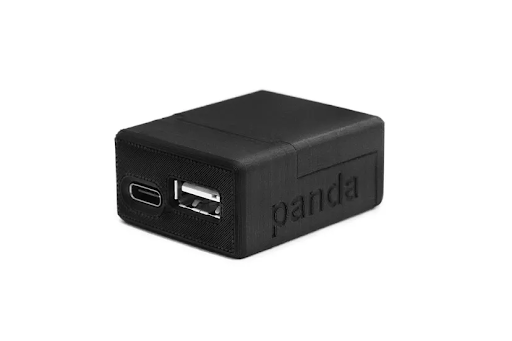
\includegraphics[scale=0.5]{Assets/panda.png}\\
    \caption{The most pretty panda yet [1].}
    \label{fig:enter-label}
\end{figure}
This is the panda interface system that allows openpilot to send the information collected from the peripherals to be transferred to the car. It also allows the comma device to connect to the vehicle [1].




\section{Architecture}
\subsection{High-Level OpenPilot Architecture}
    In general, OpenPilot can be depicted as a layered style architecture which contains 8 layers.
    \begin{itemize}
        \item[] Layer 1: Vehicle Interface 
        \item[] Layer 2: Communication and Data Interpretation
        \item[] Layer 3: Sensing and Actuation
        \item[] Layer 4: Core Neural Network Runners
        \item[] Layer 5: Localization and Calibration 
        \item[] Layer 6: Control Algorithms
        \item[] Layer 7: System Management and Logging
        \item[] Layer 8: User Interface and Experience 
    \end{itemize} 
    \begin{figure}[ht]
        \centering
        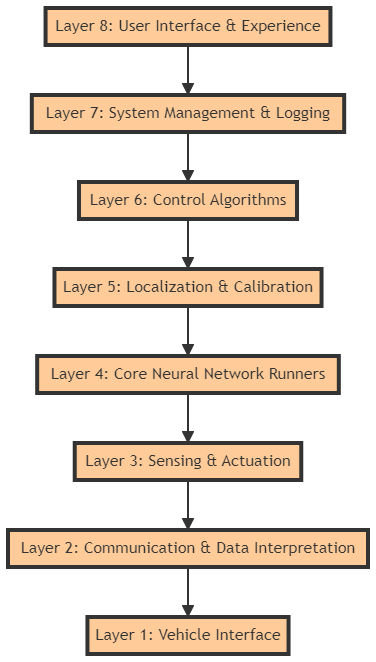
\includegraphics[scale=0.15]{Assets/layers.png}\\
        \caption{A bottom up diagram detailing the conceptual architecture of openpilot}
        \label{fig:enter-label}
    \end{figure}

    \begin{itemize}
        \item The \textbf{vehicle interface layer} includes the car’s hardware and peripherals that interface with OpenPilot. This includes \textbf{CAN} interface which enables communication with the car’s internal network, \textbf{steering wheel angle} sensor measures angle of steering wheel, \textbf{camera} provides visual input around the vehicle, \textbf{IMU} also provides movement and orientation information, \textbf{GNSS Receiver} provides global positioning data, and along with other vehicle sensors that are used to ensure the vehicle is functioning properly [5].
    
        \item The \textbf{communication and data interpretation layer} consists of libraries like opendbc which interprets CAN bus data based on \textbf{DBC} files, \textbf{panda} which is hardware that is used to read/write from and to the CAN bus, \textbf{laika} which processes \textbf{GPS} data for more precise positioning, and \textbf{cereal} which is the message protocol for inter-process communication [5].
        
        \item The \textbf{sensing and actuation layer} includes \textbf{boardd} which manages communication between the panda and the openpilot software, \textbf{camerad} which processes image data from the car’s cameras, and \textbf{sensord} which handles IMU and additional sensor data reading. All together this layer manages the direct interaction with the car’s hardware and the data from the sensors [5].
        
        \item The \textbf{core neural network runners layer} includes \textbf{modeld} which runs the driving policy in order for the neural network to make driving decisions, \textbf{dmonitoringmodeld} which runs the driver monitoring neural network to ensure that the driver is paying attention, \textbf{dmonitoringd} which contains logic to see whether the driver can take over the wheel if necessary. Overall, this layer runs the neural networks which are responsible for driving and driver monitoring [5].
        
        \item The \textbf{localization and calibration layer} includes \textbf{ubloxd} which parses GNSS data for localization, \textbf{locationd} which uses a Kalman filter service to provide precise vehicle localization, \textbf{calibrationd} which calibrates the camera to align it with the vehicle’s frame, and \textbf{paramsd} which adjusts the vehicle parameters for more accurate control [5].
        
        \item The \textbf{control algorithms layer} uses \textbf{radard} which processes radar data for detecting objects and tracking them, \textbf{plannerd} which laterally and longitudinally calculates the path planning, and \textbf{controlsd} which generates and sends the control commands to the actuators of the vehicle [5].

        \item The \textbf{system management and logging layer} contains \textbf{manager} which oversees the lifecycle of openpilot services, \textbf{thermald} which monitors the thermal state of the device and ensures it does not overheat, \textbf{loggerd} which records driving and analyses that data for improvements, \textbf{logcatd} which logs system messages and errors, \textbf{proclogd} which logs detailed process data, and \textbf{athenad} which manages the connection to common.ai services for updates and any remote assistance [5].
        
        \item Lastly, \textbf{the user interface and experience layer} has a \textbf{UI} which is in charge of displaying the interface for the user, including a live camera feed, system alerts and status [5].  

    
        
    \end{itemize}

\subsection{Derivation}
  
    This conceptual high-level layered architecture diagram was derived by reviewing comprehensive details about the openpilot architecture, understanding each of the components, functionalities, and how they interact with each other. Organizing the layered architecture into eight layers is crucial in creating a hierarchical structure for modularity, debugging, and understanding the flow of data. Each layer consists of the specific components that perform the layer’s function. This includes the hardware interfaces, libraries used for data processing, neural networks, localization services, control algorithms, system management tools, and user interface elements. A rectangle box was used to capture each layer and arrows were used to show connections to indicate the flow of data and commands between the layers. 

\subsection{Global control flow}

    In Figure 3, the control flow of the system is divided into it's subsystems with the following groups: Sensors and Actuators, Location/Calibration, Neural Network Runners, Controls, and System Management.

    \begin{itemize}
        \item All messages to and from the panda are managed by boardd [4]
        boardd acts as a publisher for other systems to observe messages from the panda [4]

        \item radard publishes a radarState based on the information received from modeld and boardd [4]

        \item plannerd uses the radarState object to make its path, then publishes said path [4]

        \item controlsd takes the published path and converts it into CAN commands, it then sends those commands back to boardd, so that boardd can send them back to the panda device [4]

        \item camerad captures and publishes video from the cameras [4]

        \item modeld transforms the video with a machine learning model and publishes the result [4]

        \begin{figure}[ht]
        \centering
            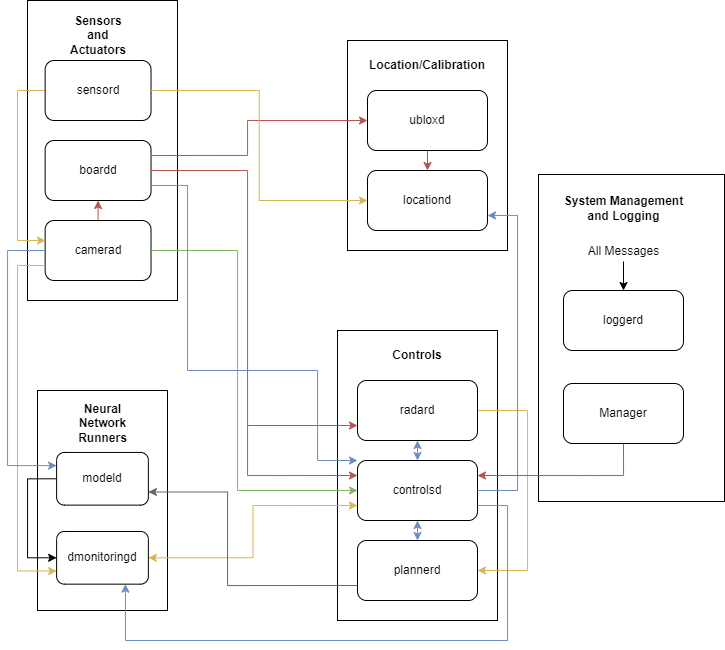
\includegraphics[scale=0.35]{Assets/global_control_flow.png}
            \caption{A control flow diagram of openpilot}
            \label{fig:enter-label}
        \end{figure}

    \end{itemize}

\newpage
\subsection{Alternative architectures}

    \begin{itemize}
        \item[] \textbf{Pipe and filter}

        \begin{figure}[ht]
        \centering
            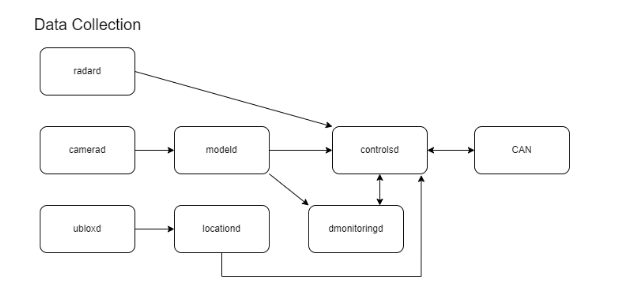
\includegraphics[scale=0.7]{Assets/pipeandfilter.PNG}
            \caption{Pipe and filter diagram for openpilot}
            \label{fig:enter-label}
        \end{figure}
         Figure 4 shows an extremely simplified higher level diagram  to represent an alternative
         pipe and filter architecture. This was derived from the control flow diagram and showcases the flow of data as successive streams from one direction to the other The system collects data from the car's sensors, including cameras and radars, as well as GNSS (Global Navigation Satellite System) data for localization. The camerad service captures video frames, while radard processes radar data, and ubloxd handles GNSS data. The captured data is then processed and analyzed to understand the current driving environment. The neural network, running within the modeld service, analyzes camera frames to predict driving paths and detect obstacles, lane lines, and other relevant features. The locationd service, using data from ubloxd, localizes the vehicle in the world. The controlsd service receives all of this and translates it into specific control commands for the vehicle. These commands are then sent to the vehicle's control systems via the Controller Area Network bus. Throughout this process, the dmonitoringd service continuously monitors the driver's state to ensure they are attentive and capable of taking over when necessary.

         \item[] \textbf{Client-server}
         \begin{figure}[ht]
        \centering
            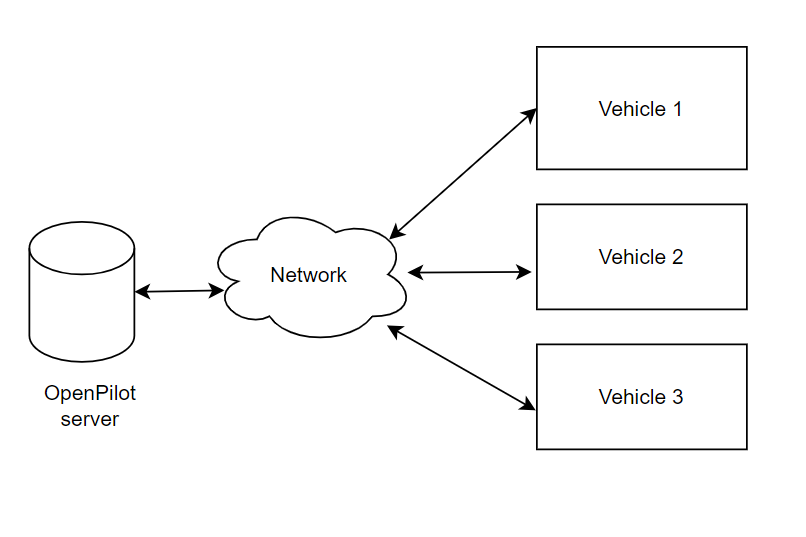
\includegraphics[scale=0.7]{Assets/clientserver.png}
            \caption{Client server diagram for openpilot's network interactions}
            \label{fig:enter-label}
        \end{figure}

        OpenPilot automatically sends collected driving data to its servers, where this data pool is used to train and refine its machine learning models. This showcases a classic client-server framework, with the server housing the data and the Comma device within the vehicle acting as the client that communicates data over network connections [5]. In this model, standalone servers are interfaced by clients via a network, highlighting the interconnected roles of the server and client in the system architecture.
    \end{itemize}



\subsection{Evolvability}

    OpenPilot continuously improves through a combination of data collection, machine learning based on that data, and contributions from the open-source community [2]. By logging sensor inputs, control commands, and vehicle responses, OpenPilot can train and enhance its neural network models, leading to incremental improvements in the system's overall performance [4]. Moreover, the collaborative nature of its development means that new features, bug fixes, and code optimizations from community contributors are regularly incorporated, enriching the project. With each new release, OpenPilot rolls out additional features. For instance, the latest version has an upgraded driving model with superior navigation performance, support for a wider range of car models, and more sophisticated lateral planning algorithms [2].
    
\subsection{Concurrency}
    \begin{itemize}
        \item[] \textbf{Concurrent testing}: Utilises the \textbf{pytest} module to achieve parallelization and streamline test suite execution. This allows for concurrent testing, maximising resource use and minimising idle time [2]. 
        \item[] \textbf{Driving controls system}: The control system handled by the \textbf{controlsd} module is responsible for managing autonomous vehicle operations, it relies on concurrent data from other modules and is responsible for executing crucial driving functions including acceleration, braking, and steering [2].
        \item[] \textbf{Driver monitoring system}: The driver monitoring system handled by the \textbf{dmonitoringd} is responsible to ensure the driver remains alert, It ensures driver attentiveness and readiness to take control when necessary. It concurrently processes data provided by a machine learning model, and video data to decide if the driver needs to be alerted [2].

    \end{itemize}



\subsection{Division of responsibilities}%%FINISH THIS

There are a division of responsibilities among developers for the openpilot system that have to be met in order to ensure that the system is running smoothly. 

    \begin{itemize}
        \item[] \textbf{Specialization and Expertise Development}: Developers focus on their areas of expertise, like machine learning or sensor integration, improving code quality and fostering innovation within their domains.
.

        \item[] \textbf{Collaboration and Integration}: Effective inter-service communication and collaborative testing are essential to ensure well-defined interfaces and system-wide debugging.


        \item[] \textbf{Scalability and Maintenance}: Modular development promotes easier updates and maintenance, while knowledge sharing ensures continuity even if key developers are unavailable.

    

        \item[] \textbf{Challenges}: Managing dependencies and communication overheads are significant challenges due to the division of responsibilities among services.


        \item[] \textbf{Continuous Integration and Deployment}: CI/CD pipelines which are automated processes in software development that enable teams to frequently deliver code changes are crucial for managing complexity, automating testing, and ensuring seamless deployment across the system.


        \item[] \textbf{Open Source Community Engagement}: Engaging with the community expands the project through contributions and feedback, but requires coordination to align with project standards.

    \end{itemize}



\subsection{Important architectural styles and design patterns}

While not explicitly stated in its documentation, based on OpenPilot’s architecture and functionality, we can infer the use of the following design patterns:

\begin{itemize}

    \item \textbf{Design patterns used}
    \begin{itemize}
         \item[] \textbf{Observer pattern}: OpenPilot likely uses the Observer pattern for handling sensor data and state changes within the vehicle's system. Sensors, cameras, radars, and GPS continuously generate data and the Observer pattern would allow various components of OpenPilot (observers) to subscribe to this data and be notified of changes, enabling real-time responses to sensor inputs [5].

    \item[] \textbf{Model View Controller (MVC)}: The separation of the system's user interface from its logic and data models suggests the use of the MVC pattern. This is particularly relevant in the context of OpenPilot's GUI, where the interface (View) displays information based on vehicle data (Model), managed by system logic (Controller).

    \item[] \textbf{Client-server pattern}: OpenPilot uses a Client-Server architecture for updates and data sharing, where the vehicle acts as the client that communicates with a central server (or cloud infrastructure). This pattern is used for  updates, collecting data, and providing remote support [5].

    

    \item[] \textbf{Factory pattern}: To handle the creation of different components or objects based on the vehicle model or configuration, OpenPilot might use the Factory pattern [4]. This allows the system to instantiate objects at runtime based on specific criteria, ensuring compatibility and customization for various vehicle models.
    \end{itemize}

    \item \textbf{Architectural styles used}
    \begin{itemize}
        \item The software utilizes an \textbf{implicit invocation} architecture which can be found in their use of cereal; comma.ai's own open source library for robotic message communication. It is also used in the boardd class which acts as the "publisher". The class manages messages sent/received to/from the panda module.
        \item The previously discussed \textbf{pipe and filter} architecture is also used.
        \item The previously discussed \textbf{layered} architecture is also used in abstraction and separation of components. From sensors and actuators, software components, panda and CAN bus.
        
    \end{itemize}
\end{itemize}

\subsection{Dependencies}

\begin{figure}[ht]
    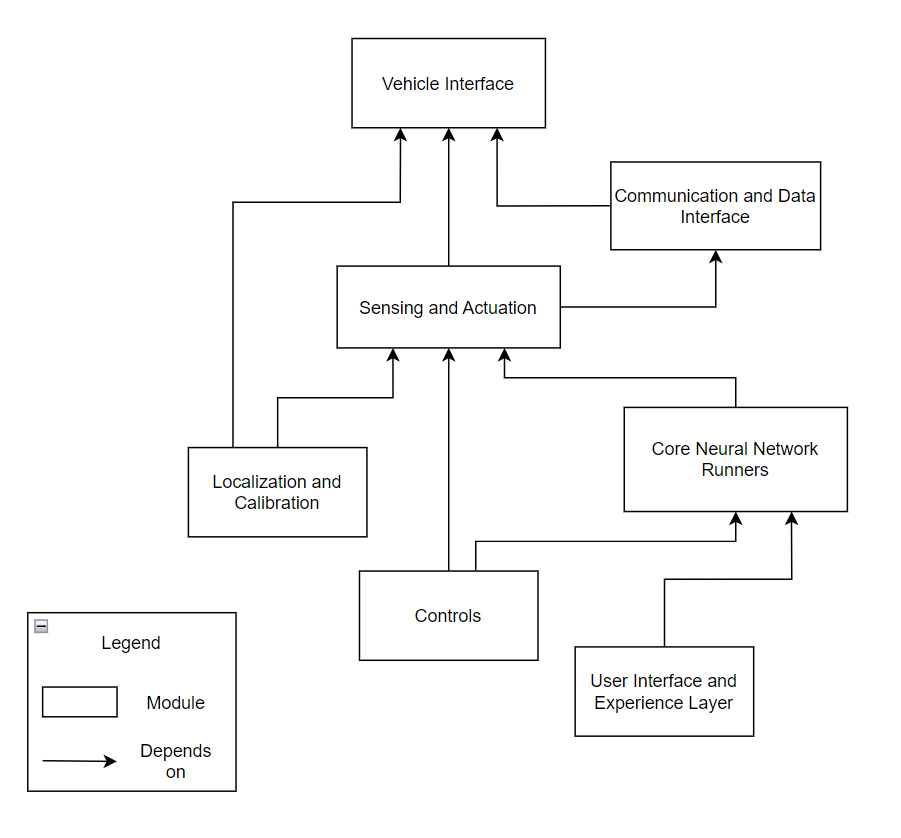
\includegraphics[scale=1]{Assets/dependencies.png}
    \centering
    \caption{A dependency diagram illustrating openpilot's component dependencies}
    \label{fig:enter-label}
\end{figure}

\begin{itemize}
    \item \textbf{Communication and Data Interpretation Layer} depends on the Vehicle Interface Layer for raw data from the car's hardware.
    \item \textbf{Sensing and Actuation Layer} relies on the Communication and Data Interpretation Layer for interpreted data (e.g., CAN messages, GPS data) to interact with the vehicle’s hardware and sensors and also relies on raw data from the Vehicle Interface Layer for direct sensor access.
    \item \textbf{Core Neural Network Runners Layer} depends on processed sensor data from the Sensing and Actuation Layer to make driving decisions and monitor the driver's state.
    \item \textbf{Localization and Calibration Layer} depends on the Vehicle Interface Layer for raw GNSS and other sensor data for localization and processed sensor data from the Sensing and Actuation Layer for precise localization and calibration.
    \item \textbf{Control Algorithms Layer} depends on sensor data from the Sensing and Actuation Layer for object detection and tracking as well as outputs from the Core Neural Network Runners Layer to make path planning and control commands.
    \item \textbf{User Interface and Experience Layer} relies on decision data from the Core Neural Network Runners Layer to provide user feedback and display critical information.
\end{itemize}

\section{External Interfaces}

In OpenPilot, different types of information are transmitted to and from the system through different interfaces and protocols. Some of the content transmitted to/from the system includes:

\begin{itemize}
    \item \textbf{Graphical User Interfaces (GUIs)}
    \begin{itemize}
        \item To the System: 
        \begin{itemize}
            \item[] User preferences and settings such as adjusting the adaptive cruise control or lane-keeping assist [4]. 
            
            \item[] Manual overrides or commands such as disengaging autopilot or manually adjusting the set speed [4].
        \end{itemize}
        

        \item From the System: 

        \begin{itemize}
            \item[] Real-time vehicle data such as speed, acceleration, etc [4].
            \item[] Camera feeds and sensor data visualizations [4].
            \item[] Navigation and route information [4].
        \end{itemize}
    \end{itemize}

    \item \textbf{Files}
    \begin{itemize}
        \item To the system:
        \begin{itemize}
            \item[] Configuration files containing vehicle-specific parameters and settings [4].
            \item[] Firmware and software updates [1].

        \end{itemize}

        
        \item From the system:

        \begin{itemize}
            \item[] Log files with driving data, system errors, etc [5].
            \item[] Recorded sensor data such as camera footage, radar readings for analysis [4].
 
        \end{itemize}
        
    \end{itemize}

    \item \textbf{Messages or networks}

    \begin{itemize}
        \item To the system:
        \begin{itemize}
            \item[] Control commands and signals within the system [5].
            \item[] Commands or updates from the server [1].

            
        \end{itemize}

        
        \item From the system:

        \begin{itemize}
            \item[] Data sent to servers for analysis, improvement, and support [5].
            \item[] Alerts and notifications to the user's mobile device or web interface [5].
 
        \end{itemize}
    \end{itemize}
\end{itemize}








\section{Use Cases}

This is a sequence diagram that shows the workflow for determining if it's safe to engage the open pilot system.
First of all, when the user starts up tries to start up the openpilot system, it goes through the manager service which has to check if it's actually safe to engage the system and engage it if it is safe. The manager service uses the dmonitoringd service to determine if it is safe to engage the system. To do this, first, the dmonitoringd service checks to see if the user has been distracted for extended periods of time. If so, it deems it unsafe, and prevents the user from enabling the openpilot system. Otherwise, it uses a combination of user alertness information that's gotten from the user facing camera, as well as scene information that’s gotten from the driving model, to either determine whether it's safe to engage the system or whether to alert the user if they are distracted.


\begin{figure}[ht]
    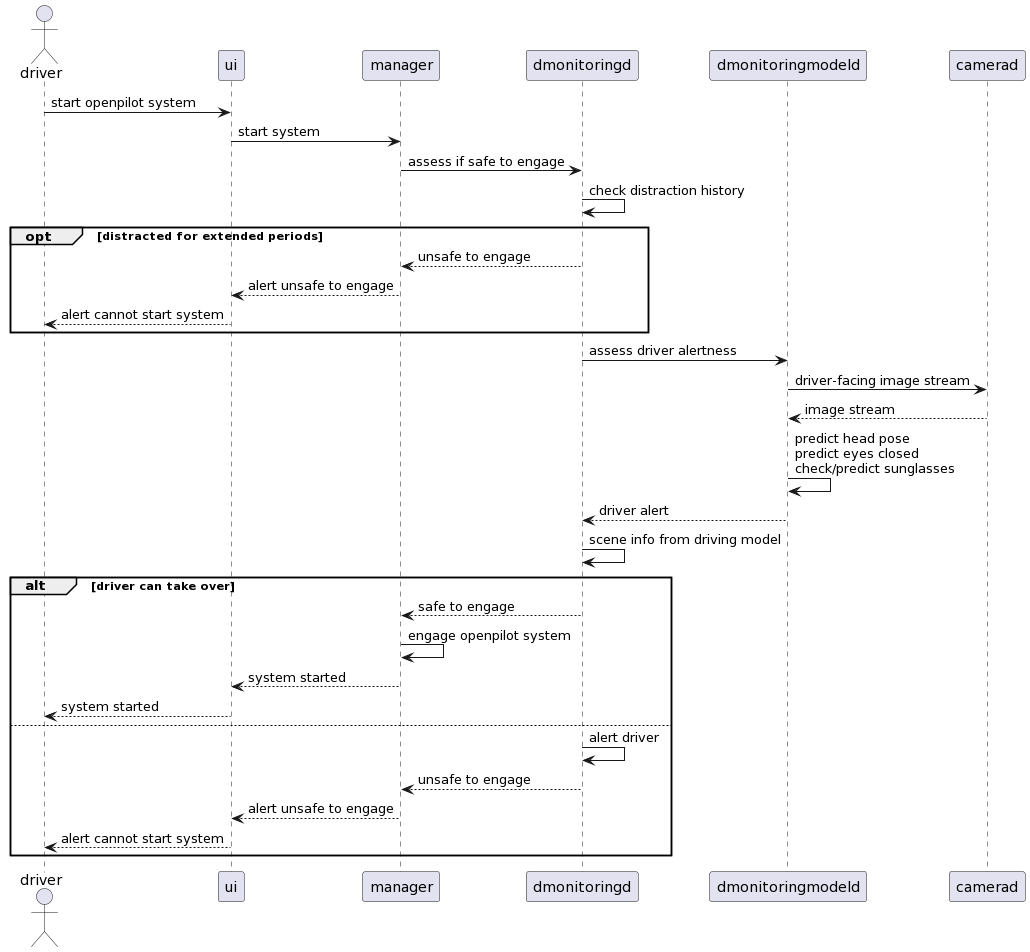
\includegraphics[scale=0.15]{Assets/sequence.png}
    \\
    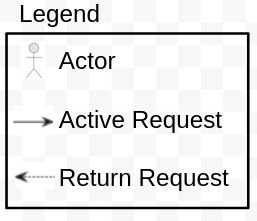
\includegraphics[scale=0.15]{Assets/legend.png}
    \centering
    \caption{A use case diagram detailing a case where a driver becomes distracted while openpilot is active}
    \label{fig:enter-label}
\end{figure}


\begin{figure}[ht]
    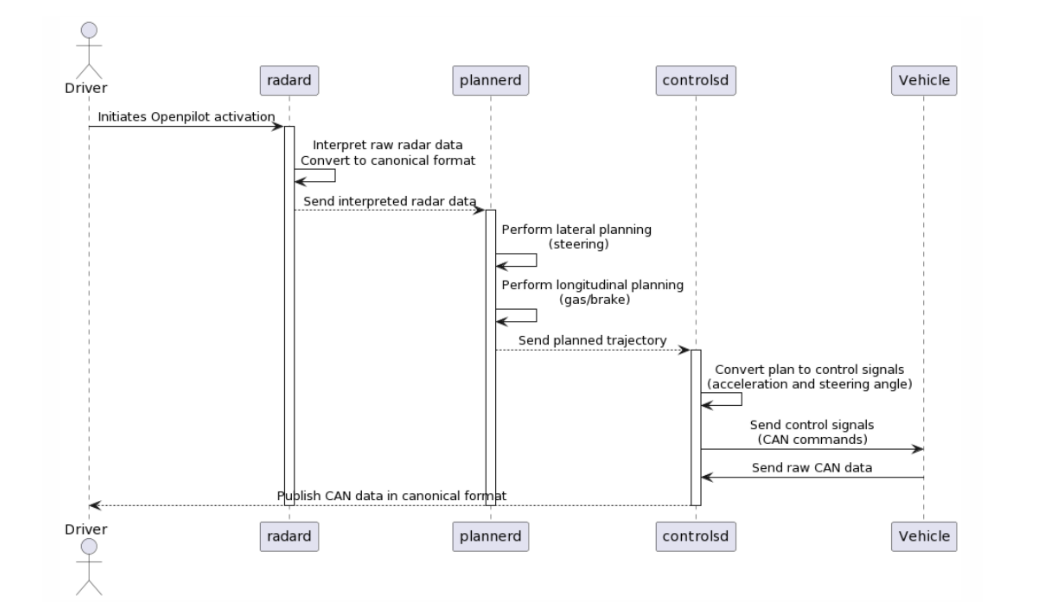
\includegraphics[scale=0.3]{Assets/usecase.png}
    \centering
    \caption{A use case diagram detailing a case where a driver uses openpilot regularly}
    \label{fig:enter-label}
\end{figure}

The second use case is for a scenario where the driver initiates openpilot and subsequently radard detects objects around the vehicle. The radard component then converts the object data around the car into canonical format and sends the data to plannerd which will decide which direction to steer the vehicle. It will also decide whether to accelerate or decelerate depending on the situation.These decisions are sent to controlsd to execute the functions such as steering/acceleration and deceleration, to which the vehicle will make the physical movements.
\newpage
\section{Data Dictionary}

    \begin{itemize}

        \item[] \textbf{comma three}: The device mounted in the car that the driver interacts with. It has an integrated panda within the system. Comma three runs on a Ubuntu based operating system [5]. It contains three HDR cameras, two to watch the road and one night vision camera to point inside of the car to watch the driver. This assists with the driver attentiveness system [6].
        \item[] \textbf{CAN Bus}: Message based protocol that allows components of the vehicle, called Electric Control Units, to communicate with each other [7].
        \item[] \textbf{Neural Network}: The machine learning model that openpilot uses to predict where the car should go given the input from modeld [5][4].
        \item[] \textbf{GNSS}: Satellites that provide positioning, navigation, and timing services. GPS is an example of a GNSS [8].
        \item[] \textbf{cereal}: Messaging system between robotic systems. Utilizes a publisher and subscriber model [5].
        

    \end{itemize}

\section{Naming Conventions}

    \begin{itemize}

        \item[] \textbf{CAN}: Controller Area Network
        \item[] \textbf{DBC}: Database CAN
        \item[] \textbf{GNSS}: Global Navigation Satellite System
        \item[] \textbf{GPS}: Global Positioning System
        \item[] \textbf{IMU}: Inertial Measurement Unit
        \item[] \textbf{UI}: User Interface
        

    \end{itemize}

\section{Conclusion}
Overall, we were able to get a comprehensive overview of the architectural framework of OpenPilot through lengthy discussions of the various systems and subsystems that make up the system as a whole. The architecture is organized into a layered structure, connecting major systems, ranging from the user interface to the vehicle's interface layer. From layered architecture to implicit inovation, and from pipe and filter to client-server interactions, each element contributes to creating a robust, flexible, and evolving system. The focus of future studies will be to transition from conceptual to concrete architecure. Further research will be conducted in order to get a better understanding of the system that fully encompasses OpenPilot.


\section{Lessons learned and Alternatives Presented}

One lesson that was abundantly clear to the group in the making of this report was how architecture styles can manifest themselves in large scale systems such as openpilot. This report detailed how the entirety of openpilot's components and subsystems could not be confined to simply one architecture style. The layered style, pipe and filter style, and implicit invocation style were all used to capture the functionalities of the product's systems. Although it may seem obvious in hindsight, the group wishes they could have been more cognizant of how different architecture styles may be present within subsystems, yet still be able to communicate and act as a cohesive unit. If this was better known it would have remedied a lot of difficulty the group had in choosing how to represent the architecture styles.

Another lesson we learned and discussed during our presentations was that the development of autonomous driving systems such as comma.ai's Openpilot heavily relies on neural networks and machine learning algorithms to interpret and respond to complex real-world data. The lessons learned emphasize the critical importance of continuously improving AI models to ensure the safety and reliability of autonomous driving features, particularly in noisy environments. Comma.ai's approach underscores the necessity of leveraging vast amounts of data collected from vehicles equipped with Openpilot to train and refine neural network models effectively. It is imperative for comma.ai to meticulously curate and preprocess this data, accounting for various sources of noise and uncertainty inherent in real-world driving conditions. Furthermore, ongoing research and development efforts must focus on enhancing the robustness and adaptability of AI models to navigate unpredictable scenarios and mitigate the impact of environmental noise. By prioritizing data quality, model optimization, and rigorous testing methodologies, comma.ai can continue to advance the capabilities of Openpilot and deliver safer and more reliable autonomous driving experiences for users.

An essential lesson learned from studying Openpilot is the significance of delving into the intricacies of software architectural styles to gain a comprehensive understanding of the system's design and functionality. Rather than merely listing architectural styles, it is imperative that we explain and thoroughly research how they interrelate within the Openpilot ecosystem and the benefits they offer. By examining architectural styles such as pipe-and-filter and layered architecture in detail, researchers and developers can elucidate how these design principles shape the modularity, scalability, and maintainability of the system. Additionally, exploring the rationale behind the selection of specific architectural patterns within Openpilot provides valuable insights into the system's evolution, performance optimizations, and adaptability to evolving requirements. Emphasizing the importance of software architecture in the study of Openpilot underscores its foundational role in facilitating system extensibility, fault tolerance, and overall system robustness, thereby fostering a deeper appreciation of the engineering principles underpinning autonomous driving technology.


\begin{thebibliography}{00}

    \bibitem{b1} S. Anumakonda, “The state of comma.ai,” Medium.com, \url{https://srianumakonda.medium.com/the-state-of-comma-ai-2140aabc6f52} (accessed Feb. 13, 2024).

    \bibitem{b2} “openpilot 0.9.5,” comma.ai, \url{https://blog.comma.ai/095release/} (accessed Feb. 13, 2024).

    \bibitem{b3} “Openpilot - Open source advanced driver assistance system,” comma.ai, \url{https://comma.ai/openpilot} (accessed Feb. 13, 2024).

    \bibitem{b4} “From vision to architecture: How to use openpilot and live,” From Vision To Architecture: How to use openpilot and live - DESOSA 2020, \url{https://desosa.nl/projects/openpilot/2020/03/11/from-vision-to-architecture} (accessed Feb. 13, 2024).

    \bibitem{b5} “How openpilot works in 2021,” comma.ai, \url{https://blog.comma.ai/openpilot-in-2021/} (accessed Feb. 13, 2024). 

    \bibitem{b6} “Comma 3x - make driving chill,” comma.ai, \url{https://comma.ai/shop/comma-3x} (accessed Feb. 13, 2024). 

    \bibitem{b7} G. M. Smith, “What Is CAN Bus (Controller Area Network) and How It Compares to Other Vehicle Bus Networks,” dewesoft.com,
    \url{https://dewesoft.com/blog/what-is-can-bus} (accessed Feb. 14, 2024).
    
    \bibitem{b8} “Other Global Navigation Satellite Systems (GNSS),” Gps.gov, Oct. 19, 2021.
    \url{https://www.gps.gov/systems/gnss/#:~:text=Global%20navigation%20satellite%20system%20(GNSS,a%20global%20or%20regional%20basis} (accessed Feb. 14, 2024).
\end{thebibliography}

\end{document}